%************************************************
\chapter{Studies of Delayed Single Electron Signals}
\label{ch:etrains} 
%************************************************

\section{Motivation for Studying Delayed Single Electron Signals}
Delayed single electron signals, known colloquially as ``electron trains'', are a generic single electron background in dual-phase \ac{LXe} \ac{TPC}s. Proportional scintillation signals consistent with those of single electrons, being emitted regularly, are known to follow high energy depositions. These electron trains can last $O(10-100)$~ms, which is the equivalent of several event windows for most \ac{LXe} \ac{TPC}s. Single electron signals were observed and investigated by ZEPLIN \cite{Edwards2008} \cite{Santos2011}, Xenon100 \cite{Aprile2014}, and LUX \cite{Xu2016}. 

\ac{LUX} collaborator Jingke Xu investigated delayed electron signals in \ac{LUX} \cite{Xu2016}. A plot of an electron train from \ac{LUX} is shown in Figure~\ref{fig:lux_etrain}. Note that the time window is orders of magnitude greater than the \ac{LUX} event window of 400~$\mu$s, and the maximum drift time for Run03 of 300~$\mu$s. In addition to electron trains, the \ac{LUX} collaboration colloquially refers to one type of delayed electron signal as ``electron burps'' or ``e-burps''. They are characterized by the sudden emission of $O(100-1000)$ electrons. Xu noted that e-burps can be part of an electron train, but unlike electron trains in general, he found e-burps to be uncorrelated with the size of the previous event (see inset of Figure~\ref{fig:lux_etrain}). 

\begin{figure}[htbp]
\begin{center}
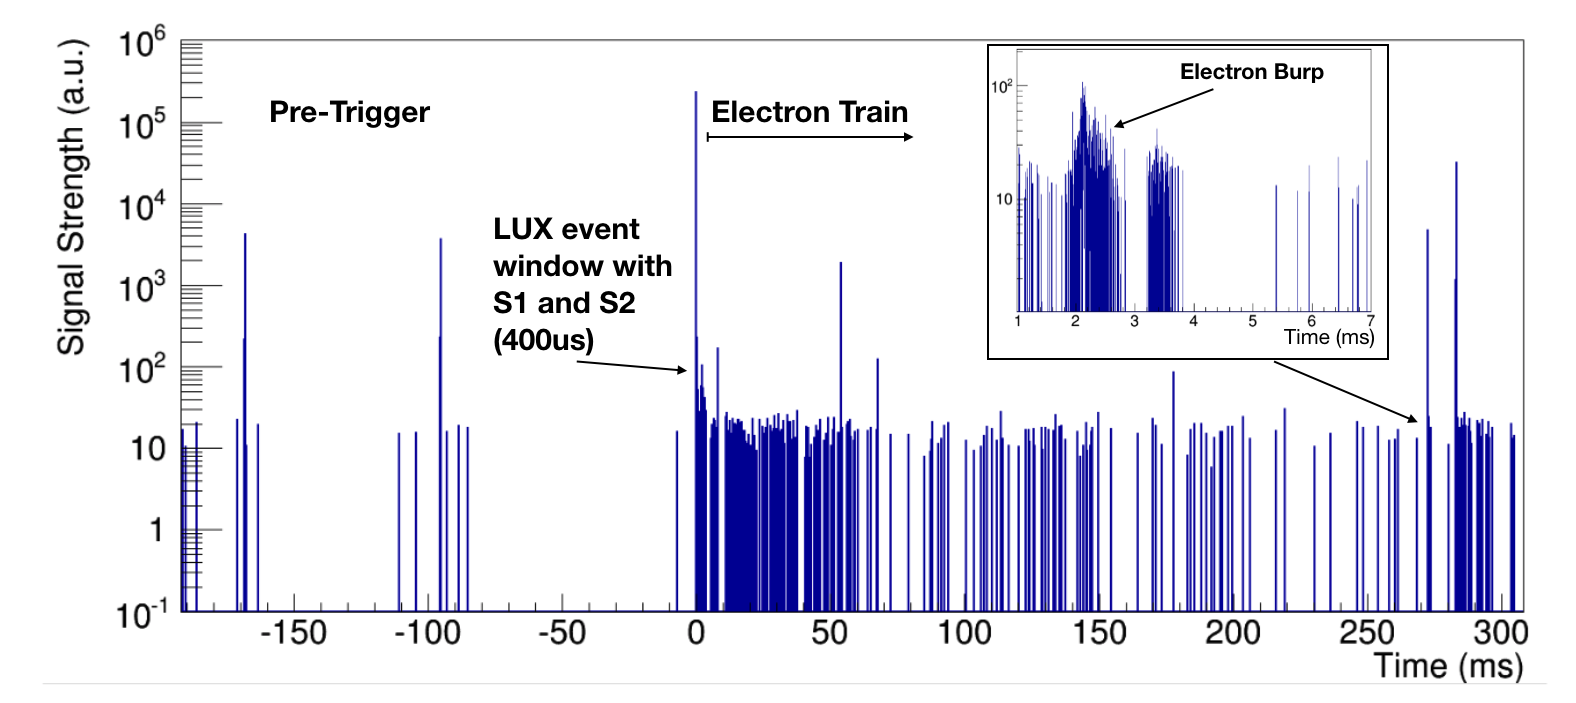
\includegraphics[width=\textwidth]{figures/etrains/lux_etrain_eburp.png}
\caption{An electron train spanning several ms. Pre-trigger and electron train regions are indicated along with the \ac{LUX} event that originated the electron train. The inset shows the shorter time structure of e-burps. The y-axis is a proxy for phd/sample. Such figures of electron trains are generated from .dat files, not from .evt files. Figure courtesy of J. Xu. }
\label{fig:lux_etrain}
\end{center}
\end{figure}


In Section~\ref{sec:non_wimp_searches_with_lxetpcs}, we discussed several dark matter searches that differ from the standard \ac{WIMP} search and how they can be completed with dual-phase \ac{LXe} \ac{TPC}s. In particular, recall the Xenon10 search for low-mass \ac{WIMP}s \cite{Angle2011}. The S2-sensitive trigger threshold was set to the level of a single electron, but an analysis threshold of 4 electrons was required for S2 size. The reason behind this is illustrated in Figure~\ref{fig:xenon10_s2s}. Although single electrons following a high-energy event can be positively identified as belonging to an electron train, electron trains can last $O(10-100)$~ms. In any event window following the start of electron train, it is unknown whether the single electron is truly a small energy deposition from a low-mass dark matter event or if it belongs to an electron train. Moreover, single electrons from a train can pile up in time, creating energy depositions the size of 2 and more electrons -- so an analysis threshold of 2 electrons is not sufficient to cut out electron train backgrounds. In general, electron trains are irritating for \ac{WIMP} searches because some percentage of the detector livetime is taken up by electron train pile-up; but they greatly limit the discovery potential for low-mass searches, as the expected signal size (S2 of 2 or 3 electrons) is possibly electron train pile-up, and therefore must be considered as such.

\begin{figure}[htbp]
\begin{center}
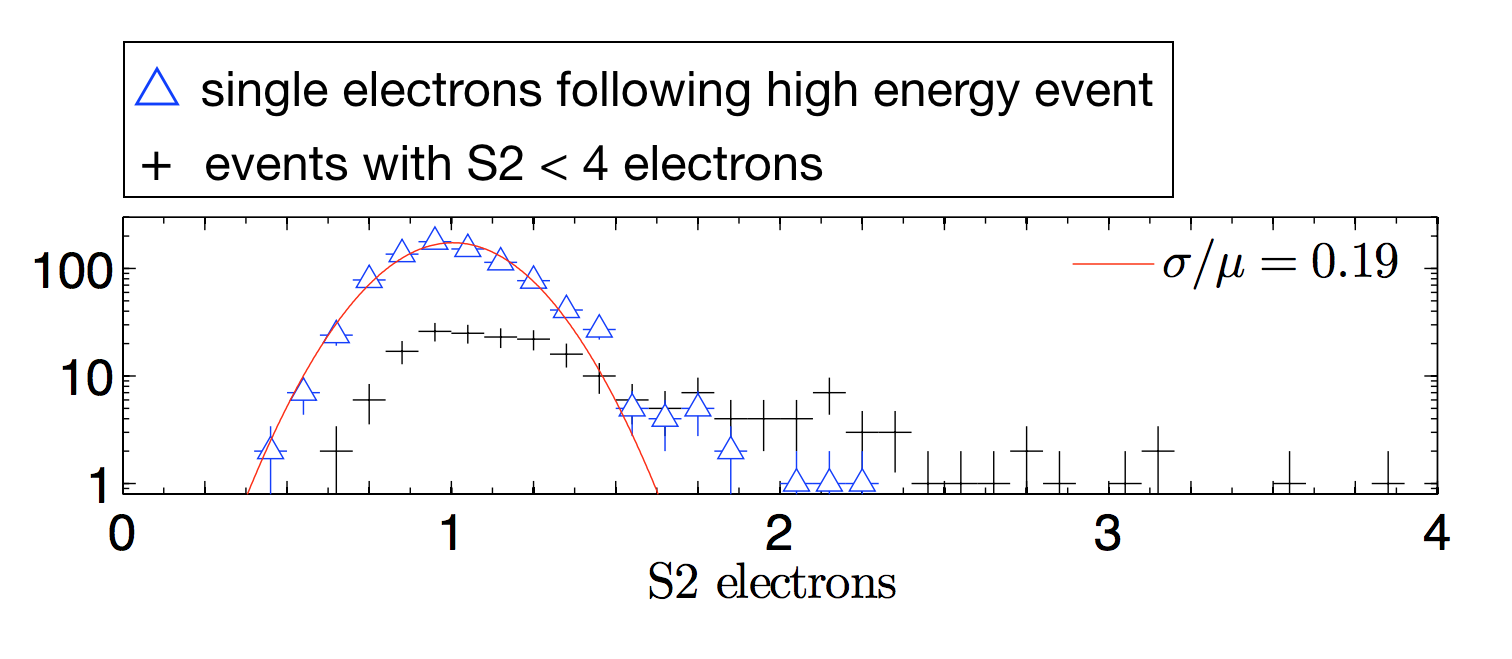
\includegraphics[width=0.9\textwidth]{figures/etrains/xenon10_s2s.png}
\caption{Figure adapted from \cite{Angle2011}.}
\label{fig:xenon10_s2s}
\end{center}
\end{figure}

Xenon100 measured the rates of 1-,2-, and 3-electron signals following an S2 \cite{Aprile2014}. They saw a relation of the time constants $\tau_{3} \approx \tau_{1}/3$ for 3-electron signals compared to 1-electron signals, and $\tau_{2} \approx \tau_{1}/2$ for 2-electron signals. They note that if multi-electron signal results from accidental time coincidences of single electrons, these time relations can be explained. 


\section{Origin of Delayed Single-Electron Signals}
While the origin of delayed single electron signals is still an area of active research, some behavior of electron trains are fairly well understood. An electron train can be split into two time regions: the primary event window ($O(100)$~$\mu$s, e.g. 400~$\mu$s in \ac{LUX}), and the following train, which continues for $O(10-100)$~ms. A few features are typically evident in the primary event window, which have origin in physical phenomena. These phenomena are discussed in the following subsections. 

\subsection{Photoionization on Grids} 
The large number of \ac{VUV} photons in big S2s are capable of liberating electrons from metallic electrodes. Electrons can be photoionized on any grid in the \ac{TPC}, but the effect is largest on the grids closest to the gas gap where the S2 is generated. Photoionized electrons from the anode aren't detected because they have essentially no space in which to proportionally scintillate. Photoionized electrons from extraction grid are directed toward the gas gap, extracted and then undergo proportional scintillation. These electrons join the S2 signal at a delay approximately equal to the distance between the extraction grid and the liquid-gas interface. Large S2s have tails that are composed of electrons photoionized from the extraction grid. 


\subsection{Photoionization of Impurities} 
Electronegative impurities in the liquid (e.g. O$_{2}$, N$_{2}$) capture ionization electrons from events as they are drifted to the gas region (e.g. O$_{2}$ binds an electron at 0.45~eV to become O$^{-}_{2}$). Just as the \ac{VUV} photons can ionize electrons from grids, they can also ionize electrons attached to impurities. Xenon100 found that the rate of single electrons in the primary event window scaled with S2 size, as well as the concentration of impurities \cite{Aprile2014} (see Figure~\ref{fig:electron_rates}). Some of the electrons in the primary event window of an electron train are now believed to come from photoionized impurities. This is supported by Xenon100 data which showed the rate of single electrons has a sharp cut off corresponding to the maximum drift time, and the the PMT hit pattern of the multi-electron signals are not localized around one PMT but rather spread over the PMT array  \cite{Aprile2014}. 

\begin{figure}[htbp]
\begin{center}
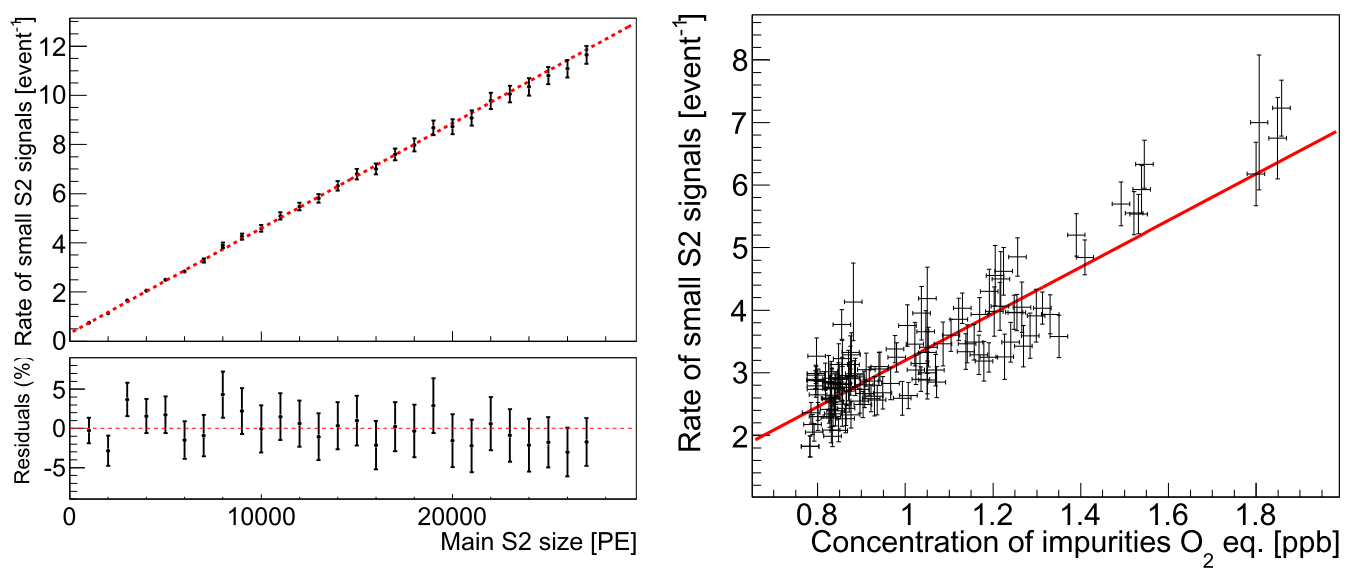
\includegraphics[width=\textwidth]{figures/etrains/electron_rates.png}
\caption{(left) The per-event rate of single electron signals 20 to 150~$\mu$s after the main S2 of a single-scatter type event as a function of the main S2 size. The fit line and residuals show a good proportionality in the relation. (right) The per-event rate of single electron signals, for events with the main S2 between 5000 and 10000 PE, as a function of the O2-equivalent concentration of impurities in liquid xenon. Figures from \cite{Aprile2014}.}
\label{fig:xenon10_s2s}
\end{center}
\end{figure}


\subsection{Delayed Extraction of Trapped Electrons} 
Dual-phase \ac{LXe} \ac{TPC}s depend on the ability to extract electrons from liquid into gas. This is accomplished with some efficiency, called the \ac{EEE}. Gushchin et al. measured the absolute \ac{EEE} in xenon and argon in 1982 as function of electric field  \cite{Gushchin1982} (see Figure~\ref{fig:eee}. Their result extends to an extraction field of 5~kV/cm in the liquid. It is common practice for modern experiments that achieve an extraction field $\gtrsim$~5keV/cm to assume they have 100\% extraction, an assumption based on the Gushchin result. Relative extraction efficiency is measured only by the size of the S2 scintillation light and inferred number of initial ionization electrons based on calibration source energy and knowledge of recombination. Relative measurements of \ac{EEE} as a function of extraction field assume 100\% extraction at the highest field and scale the other points accordingly. In contrast, absolute extraction efficiency measurements measure the number of electrons generated in the liquid as well as how many are extracted with no scaling. 

\begin{figure}[htbp]
\begin{center}
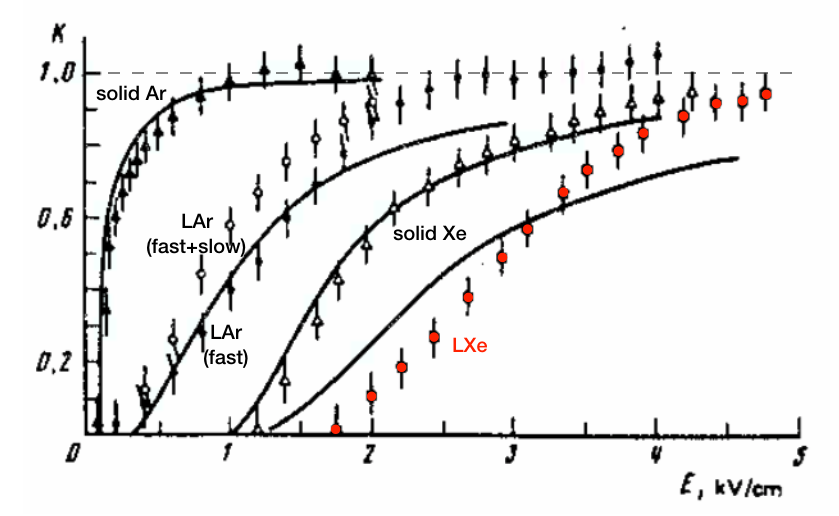
\includegraphics[width=\halffig]{figures/etrains/gushchin_eee.png}
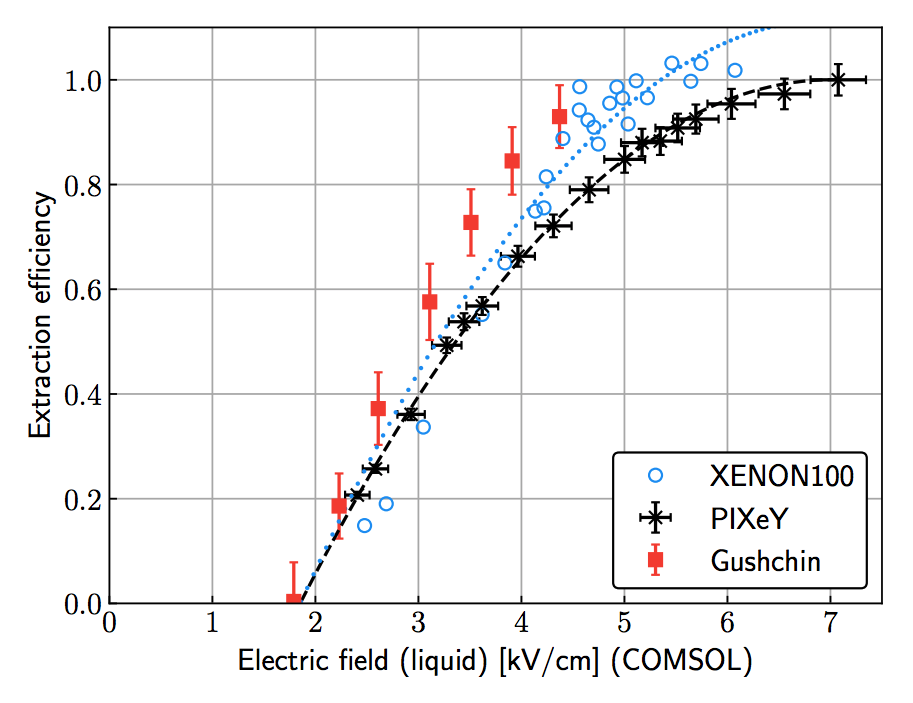
\includegraphics[width=\halffig]{figures/etrains/modern_eee.png}
\caption{(left) The absolute \ac{EEE} measured by Gushchin from \cite{Gushchin1982}. The \ac{LXe} points were re-colored red. (right) Two relative \ac{EEE} measurements from modern experiments, Xenon100 and PIXEY, compared to Gushchin. The plot is from the PIXEY result \cite{Edwards2018}, where the authors fit their result with a quadratic function ($y=ax^{2} + bx + c$). The fit to the PIXEY data (black dashed line) is scaled by a constant and applied to the Xenon100 data (blue dotted line). }
\label{fig:eee}
\end{center}
\end{figure}

Since there does not exist a second absolute measurement of \ac{EEE} out to higher extraction fields, it is uncertain when 100\% \ac{EEE} is reached in \ac{LXe}. However, it is well known that the number of extracted electrons depends on the extraction field. It is thought that the unextracted electrons are liberated from the liquid surface at a later time, as constitiuents of electron trains. Xenon100 notes that 

\section{Charge Amplifier Signals}

\subsection{Radon Source}
 radon chosen because alpha signals high energy (lots of electrons -- say how many), and uniformly distributed in volume. problems: expected to be able to select mono-energetic signal w/ PMT spectrum. 
 
 probelms: PMT saturation, low signal efficiency/low trigger rate w/ bullseye -- most events happening elsewhere. had to collect data for long time, charges built up on grids, betas complicated charge spectrum further. also had big loss of charge across extraction grid, which made signals small. 
 
\subsection{Polonium Source}

\section{Experimental Configuration}

\section{Results}
See paper for results, this should contain a little more information about the causes of e-train signals. 

%*****************************************
%*****************************************
%*****************************************
%*****************************************
%*****************************************
